\documentclass{article}
\usepackage{import}
\usepackage[ruled]{algorithm2e}
\usepackage[shortlabels]{enumitem}
\usepackage{hyperref}
\usepackage{minted}
\usepackage{subcaption}
\hypersetup{
    colorlinks=true,
    linkcolor=blue,
    filecolor=magenta,      
    urlcolor=cyan,
    pdftitle={Overleaf Example},
    pdfpagemode=FullScreen,
    }
\subimport*{}{macro}

\setlength\parindent{0px}

\begin{document}
\setcounter{problem}{0}
\title{Homework \#6}
\author{
    \normalsize{AA 597: Networked Dynamics Systems}\\
    \normalsize{Prof. Mehran Mesbahi}\\
    \normalsize{Due: Mar 1, 2024 11:59pm}\\
    \normalsize{Soowhan Yi}
}
\date{{}}
\maketitle

All the codes are available at the end of the documents or here.
\url{https://github.com/SoowhanYi94/ME597}
\begin{problem}3.8
    Consider the uniformly delayed agreement dynamics over a weighted graph, specified as
    \begin{align*}
        \dot x_i(t) = \sum_{j \in N(i)} w_{ij} (x_j(t - \tau) - x_i (t-\tau))
    \end{align*}
    for some $\tau > 0$ and $i = 1, \cdots n$. Show that this delayed protocol is stable if 
    \begin{align*}
        \tau < \frac{\pi}{2\lambda_n(G)}
    \end{align*}
    where $\lambda_n(G)$ is the largest eigenvalue of the corresponding weighted Laplacian. Conclude that, for the delayed agreement protocol, there is a tradeoff between faster convergence rate and tolerance to uniform delays on the information-exchange links.

    As we have sum of inputs ($\sum_{i \in V(i)} \dot u_i(t) = 0$) equal to 0, we know that the average of agent values are invariant set of quantities, therefore reaching average-consensus. Now, the Laplacian transform of this agreement protocol can be written as
    \begin{align*}
        X(s) = (sI + L(s))^{-1} x(0)
    \end{align*}
    where the $L(s)$ is Laplacian transform of weighted laplacian matrix. Since we know the guaranteed stability of the response, the transfer function is guaranteed to be stable. Also, we know that the transfer function involving time delay would have the time delay term $e^{-\tau s}$ in front. Therefore, the transfer function has to be stable, and the poles should be on the left hand side of the plane.
    \begin{align*}
        G(s) &= (sI + e^{-\tau s} L(s))^{-1}\\
        Z(s) &= sI + e^{-\tau s} L(s) = 0 = sI + e^{-\tau s} Q(s) \Lambda Q(s)^{-1} = 0\\
        &Q(s)^{-1} sI Q(s)+ e^{-\tau s} \Lambda = 0\\
        \therefore &sI + e^{-\tau s} \Lambda  = 0
    \end{align*}
    Using frequency domain analysis, we can substitute s with $jw$. Therefore, 
    \begin{align*}
        s & = - e^{-\tau s} \Lambda \leq 0\\
        &= -  e^{-\tau jw} \Lambda \leq 0\\
        &= - (\cos{(-\tau w)}+ j\sin{(-\tau w)})\Lambda \leq 0\\
        &= -(\cos{(\tau w)}- j \sin{(\tau w)})\Lambda \leq 0
    \end{align*}.
    Since the real part of s should be negative, $\cos{(-\tau w)}=\cos{(\tau w)} \geq 0$. Also $\Lambda = \diag (\lambda_1, \lambda_2, \cdots, \lambda_n)$, where $0= \lambda_1 \leq \lambda_2 \leq \cdots \leq \lambda_n$. Therefore,
    \begin{align*}
        jw + e^{-\tau jw} \lambda_n= 0\\
        -jw + e^{\tau jw} \lambda_n= 0
    \end{align*}.
    Multiplying those two equations yields,
    \begin{align*}
        (w - \lambda_n)^2 + 2w\lambda_n(1-sin(w\tau)) = 0
    \end{align*}.
    Sine we know $w \geq 0, \tau \geq 0$ and $\lambda_n \geq 0$, $w = \lambda_n$ and $1 = sin(w\tau)$, and therefore, the smallest $\tau$ that satisfies above equations is
    \begin{align*}
        \tau = \frac{\pi}{2\lambda_n} 
    \end{align*}.
    Therefore if $\tau \leq \frac{\pi}{2\lambda_n}$, the delayed agreement protocol is stable.

    Also according to the Gersgorian theorum, $\lambda_n \leq 2 d_{max}(G)$, where $d_{max}(G)$ is the maximum out degree in a node of the graph. Therefore  $\tau \leq \frac{\pi}{4 d_{max}(G)}\leq \frac{\pi}{2\lambda_n}$. So we can infer that the bigger the time delay, we are allowed to have more maximum out degree in a node of the graph, and therfore affecting the degree matrix of the graph and laplacian matrix, which eventually affecting the second smallest eigenvalue  or the convergence rate of the graph in agreement protocol. Therefore there is a tradeoff between faster convergence rate and the tolerance to uniform time delay. 
\end{problem}
\begin{problem} 3.9
    A matrix M is called essentially non-negative if there exists a sufficiently large $\mu$ such that $M + \mu I$ is non-negative, that is, all its entries are non-negative. Show that $e^{tM}$ for an essentially non-negative matrix M is non-negative when $t \geq 0.$

    If M is essentially non-negative, then there exists a sufficiently large $\mu$ that $M + \mu I$ is non-negative. Let $N = M + \mu I \geq 0$. Then 
    \begin{align*}
        e^{tM} = e^{t(N - \mu I)} = e^{tN}e^{-\mu  tI}
    \end{align*}
    Since $t \geq 0$, $e^{tN} \geq 0$, and $e^{-\mu t} \geq 0$, $e^{tN}e^{-\mu t I} = e^{tM} \geq 0$
\end{problem}
\begin{problem} 3.16
    Consider a network of n processors, where each processor has been given an initial computational load to process. However, before the actual processing occurs, the processors go through an initialization phase, where they exchange certain fractions of their loads with their neighbors in the network. Specifically, during this phase, processor i adopts the load-update protocol 
    \begin{align*}
        p_i(k+1) = p_i(k) - \sum_{j \in N(i)} \omega_{ij}(p_i(k) - p_j(k))
    \end{align*}
    for $k = 0, 1, \cdots ,$ that is, it sends a fraction $\omega_{ij}$ of its load imbalance with its neighbors to each of them. What is the necessary and sufficient condition on the weights $\omega _{ij}$ in above equation such that this initialization phase converges to a balanced load for all processors when the network is (1) a path graph, (2) cycle graph (3) a star graph? 
    
    Lemma 8.1 (Necessary Condition)
    
    Let the weight matrix be $W = diag(\omega_{i,j})$ for all pairs of $(i,j) \in E$. Then it is necessary to have connected graph, and to have the absolute value of the largest eigenvalue of weighted laplacian matrix less than 2 for the networks to converge to balanced load for all processors. 

    \begin{align*}
        p_i(k+1) &= p_i(k) - \sum_{j \in N(i)} \omega_{ij}(p_i(k) - p_j(k))\\
        p(k+1) &= p(k) - L_{\omega}(G) p(k) = (I - L_{\omega})(G)
    \end{align*}
    Let $M_{\omega}(G) = (I - L_{\omega}(G))$, then
    \begin{align*}
        p(k+1) &= M_{\omega}(G) p(k) = M_{\omega}(G) ^k p(0)
    \end{align*}
    where $\Lambda = diag(\lambda_1, \lambda_2, \cdots,  \lambda_n)$ and $\lambda_i \forall i \in n$ are eigenvalues of $M_{\omega}(G)$. So, for eigenvector x,
    \begin{align*}
        &M_{\omega}(G) x = (I - L_{\omega}(G)) x = \lambda(M_{\omega}(G)) x\\
        &(I - L_{\omega}(G)- \lambda(M_{\omega}(G)) I) x = 0,\text{where } x \neq 0\\
        &I - L_{\omega}(G)- \lambda(M_{\omega}(G)) I = 0\\
        &Q^{-1} (I - L_{\omega}(G)- \lambda(M_{\omega}(G)) I) Q = 0 \text{ where Q is a eigenvector matrix} [q_1, q_2, \cdots, q_n] \\
        &\therefore \lambda(M_{\omega}(G)) = I - \lambda(L_{\omega}(G)), \Lambda(M_{\omega}(G)) = 1- \Lambda(L_{\omega}(G))\\
        &\lim_{k\rightarrow\infty}p(k+1) =\lim_{k\rightarrow\infty} \Lambda ^k p(0) =  \lim_{k\rightarrow\infty}(1- \Lambda(L_{\omega}(G)))^k p(0) 
    \end{align*}
        Therefore $|1- \Lambda(L_{\omega}(G))|$ has to be less than 1 in order for the network to converge, and the $\Lambda(L_{\omega}(G)) < 2$ has to satisfy. Finally the absolute value of largest eigenvalue of the weighted laplacian matrix of the graph has to be less than 2, then it would converge to the balanced load of all processors. Delta in original equation is omitted because it is 1 in this problem.

        Corollary 8.2 (Sufficient Condition)

        If the weights are determined as the inverse of maximum of sum of weights adjacent to the node associated with the edge, it is guaranteed to have maximum eigenvalue of weighted laplacian matrix less than 2. 
        \begin{align*}
            W_{jj} = (max{(d_{\omega}(u), d_{\omega}(v))})^{-1}
        \end{align*}
        where edge uv is the jth edge, and $W_{jj}$ is the weight associated witht the edge. 
    % If the weight matrix $W = diag(\omega_{i,j})$ for all pairs of $(i,j) \in E$, is essentially non negative and sums up to 1, then those all three graphs are guaranteed to converge to a balanced load for all processors. IF W is essentially non negative, then $e^{W}$ is nonnegative, and there exists a W that can be decomposed to combination of eigenvector matrix and eigenvalue matrix, using eigenvalue decomposition. This means that W has eigenvalues that allows convergence to the average of initial conditions of agreement protocol, as the eigenvalues of weighted laplacian matrix of the graph that connects those processors satisfies quadratic form of Lyapunov function stability criterion of convergence.

    So, in (1) a path graph, those weights would be larger going into the center of the path graph. (2) cycle graph and (3) a star graph would have the same weights in all of the edges because their nodes' that forms the edge degrees are same. 
\end{problem}

\begin{problem} 8.1
    Let $H_i , i = 1, 2, 3$, be the rows of the $3 \times 3$ identity matrix in the observation scheme $z_i = H_i$ $x + v_i$ for a three-node sensor network, observing state $x \in R^3$ . It is assumed that the nodes form a path graph and that $v_i$ is a zero-mean, unit variance, Gaussian noise. Choose the weighting matrix W (8.8) and the step size $\Delta$ in (8.20) - (8.21), conforming to the condition (8.14). Experiment with the selection of the weights for a given value of $\Delta$ and their effect on the convergence properties of the distributed least square estimation (8.20) - (8.21).
    \begin{figure*}[!h]
        \centering
        \begin{subfigure}{0.45\textwidth}
            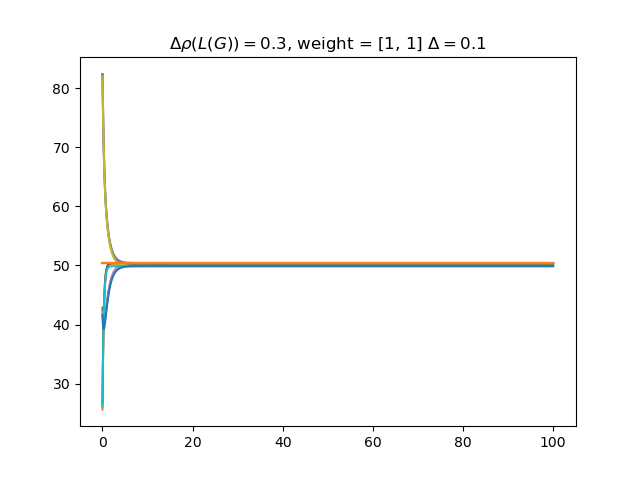
\includegraphics[width=\textwidth]{./img/Figure_0.png}
            \caption{$\Delta \rho (L(G)) = 0.3, weight = [1,1], \Delta = 0.1$}
        \end{subfigure}
        \begin{subfigure}{0.45\textwidth}
            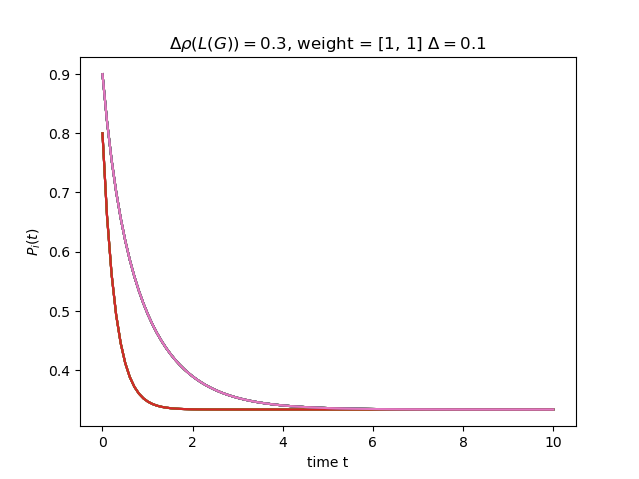
\includegraphics[width=\textwidth]{./img/Figure_1.png}
            \caption{$\Delta \rho (L(G)) = 0.4732, weight = [2,1], \Delta = 0.1$}
        \end{subfigure}
        \begin{subfigure}{0.45\textwidth}
            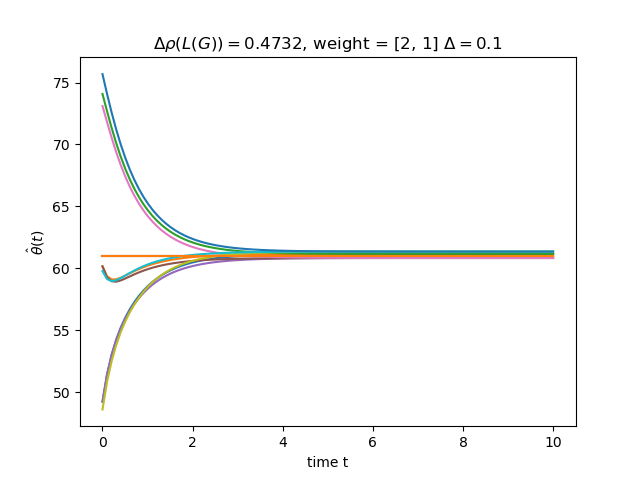
\includegraphics[width=\textwidth]{./img/Figure_2.png}
            \caption{$\Delta \rho (L(G)) = 0.6646, weight = [3,1], \Delta = 0.1$ }
        \end{subfigure}
        \begin{subfigure}{0.45\textwidth}
            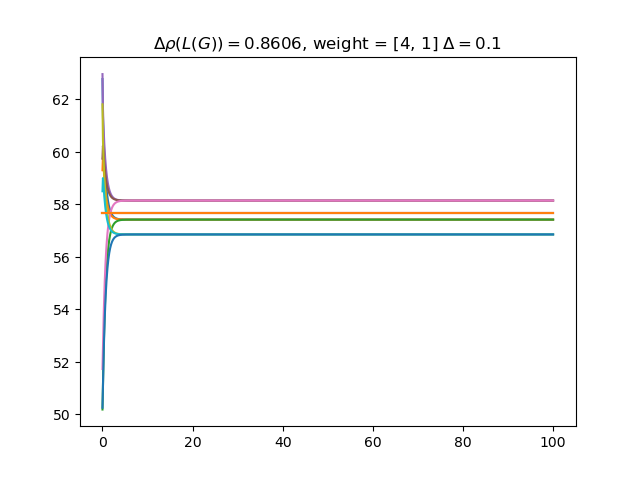
\includegraphics[width=\textwidth]{./img/Figure_3.png}
            \caption{$\Delta \rho (L(G)) = 0.8606, weight = [4,1], \Delta = 0.1$}
        \end{subfigure}
    \end{figure*}
    \newpage
    \begin{figure*}[!h]
        \centering
        \begin{subfigure}{0.4\textwidth}
            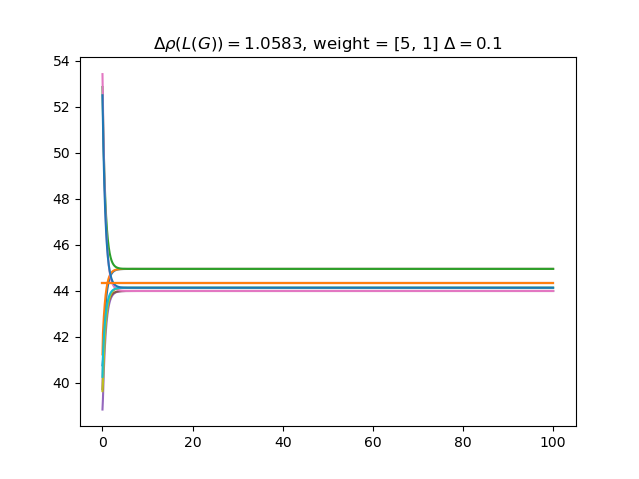
\includegraphics[width=\textwidth]{./img/Figure_4.png}
            \caption{$\Delta \rho (L(G)) = 1.0583, weight = [5,1], \Delta = 0.1$}
        \end{subfigure}
        \begin{subfigure}{0.4\textwidth}
            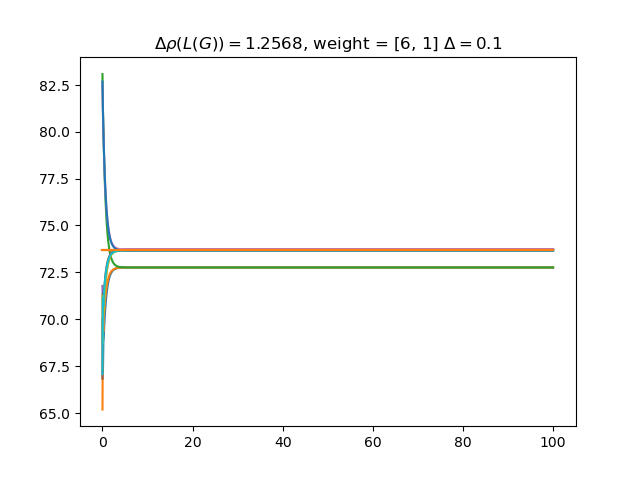
\includegraphics[width=\textwidth]{./img/Figure_5.png}
            \caption{$\Delta \rho (L(G)) = 1.2568, weight = [6,1], \Delta = 0.1$ }
        \end{subfigure}
        \begin{subfigure}{0.4\textwidth}
            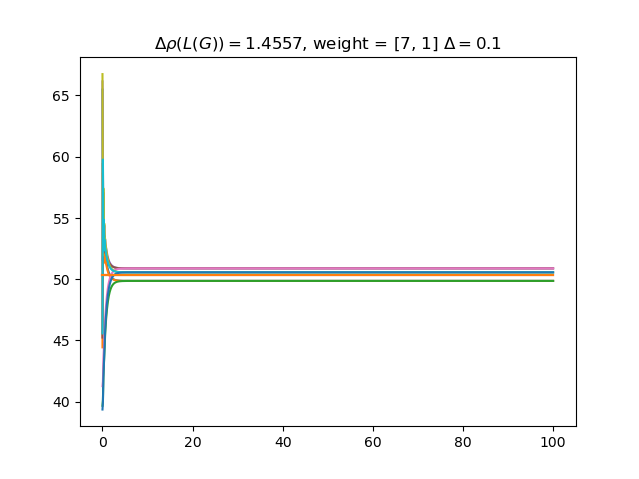
\includegraphics[width=\textwidth]{./img/Figure_6.png}
            \caption{$\Delta \rho (L(G)) = 1.4557, weight = [7,1], \Delta = 0.1$}
        \end{subfigure}
        \begin{subfigure}{0.4\textwidth}
            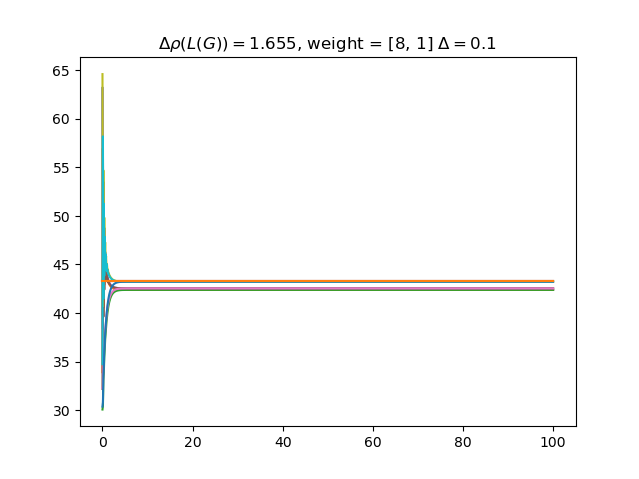
\includegraphics[width=\textwidth]{./img/Figure_7.png}
            \caption{$\Delta \rho (L(G)) = 1.655, weight = [8,1], \Delta = 0.1$}
        \end{subfigure}
        \begin{subfigure}{0.4\textwidth}
            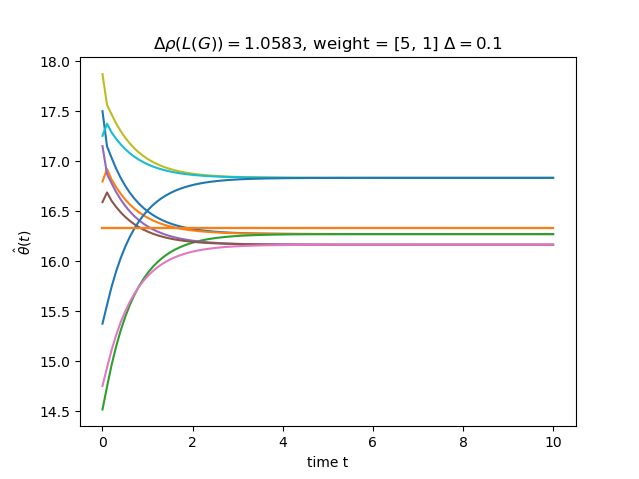
\includegraphics[width=\textwidth]{./img/Figure_8.png}
            \caption{$\Delta \rho (L(G)) = 1.8544, weight = [9,1], \Delta = 0.1$ }
        \end{subfigure}
        \begin{subfigure}{0.4\textwidth}
            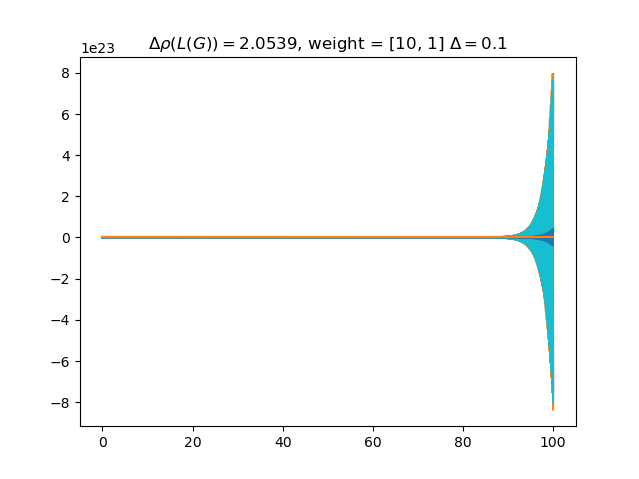
\includegraphics[width=\textwidth]{./img/Figure_9.png}
            \caption{$\Delta \rho (L(G)) = 2.053, weight = [10,1], \Delta = 0.1$ }
        \end{subfigure}
    \end{figure*}

    As we can see from those experiments, if there is significant disproportion in weights, then $\Delta \rho (L(G))$ starts increasing and their values starts to diverge as it gets bigger than 2. 
\end{problem}
\newpage
\begin{problem} 10.8
    If the network is connected, then the followers will end up (asymptotically) at
    \begin{align*}
        x_f = -A_f^{-1} B_f x_l
    \end{align*}
    given the static leader positions $x_l$ . Show that each component of $x_f$ above is in fact given by a convex combination of the components of $x_l$ .

    By definition, a convex combination of the components of $x_l$ is $\sum_{i\in l}\alpha_i x_{l_i}$ where $\sum_{i\in l} \alpha_i = 1$ and $\alpha_i \in R_+ $. Since we know that the connected network has positive definite $A_f$, it is invertible and inverted matrix would also be positive definite. Now we just need to show if all the components in $B_f$ matrix is negative or 0, and which are. As we have $D = [D_f; D_l]$, $B_f = D_f D_l^T$, therefore each entries of $B_f$ will be negative if and only if the follower corresponding to that entry is connected to some leaders. I think the each entries might be the negative of number of connected leaders to that corresponding follower. If that specific follower is not connected to the leaders, then the entries would be 0. Therefore, for connected graphs, at least one of the follower has connection with the leader, and we can conclude that each entries of $B_f$ is either negative or 0. Finally, by definition, each component of $x_f$ is convex combination of the components of $x_l$, because $A_f$ are positive definite, and each entries of $B_f$ is either negative or 0.  
\end{problem}
\begin{problem} 10.9
    Consider the linear-quadratic optimal control problem
    \begin{align*}
        \min_{u} \int_{0}^{\infty} (u(t)^T R u(t) + x(t)^T Q x(t))dt
    \end{align*}
    where the matrices Q and R are, respectively, positive semidefinite and positive definite, and 
    \begin{align*}
        \dot x(t) = -A_f x(t) - B_f u(t) 
    \end{align*}
    corresponds to a controllable network.

    Now, just because the followers execute a decentralized control strategy it does not follow that the leaders’ optimal control strategy will be decentralized. Determine if this is the case for this infinite horizon optimal control problem.
\end{problem}

\end{document}